%----------------------------------------------------------------------------------------
% KENMERKEN EN GRAFISCH OPLOSSEN. Alle opgaven zijn eigen werk.
%
% Opbouw: Probleem, Start, leerstof, en op een nieuwe pagina de Opdrachten en Test jezelf (geen Koppel in de 2de graad).
% Labels van dit hoofdstuk beginnen met h3-.
% Verschillen per pakket: relatief en absoluut extremum, een opdracht met een parameter en een bewijs, alleen in pakket 5.
% Het leerplan (LPD 20-21 in pakket 1-3, LPD 24-25 in 4-5) is in pakket 1-4 gelijk.
%----------------------------------------------------------------------------------------

\mychapter{3}{Kenmerken en grafisch oplossen}

\begin{probleem}
Op een koude winterdag meet een weerstation elk uur de temperatuur. De grafiek toont de temperatuur $T$ (in $^\circ$C) in functie van het uur $t$, van middernacht tot middernacht. Hoe laat was het het warmst, en hoe warm was het toen? Hoeveel uur vroor het die dag? En een fietser vindt het pas aangenaam vanaf $3\,^\circ$C: hoe lang was het warmer dan dat? Op de grafiek staat het antwoord, maar hoe lees je het precies af, en hoe schrijf je het kort op?

\figuren{\begin{tikzpicture}[x=.42cm,y=.42cm]
  \rooster[$t$ (h)][$T$ ($^\circ$C)]{0}{2}{24}{-4}{1}{6}
  \oorsprong
  \doorpunten{(0,1) (2,0) (4,-2) (6,-3) (8,-2) (10,0) (12,3) (14,5) (16,3) (18,1) (20,0) (22,-1) (24,-1.5)}
  \punt{0}{1}\punt{24}{-1.5}
\end{tikzpicture}}
\end{probleem}

\lkr{Leerplan \pakketnaam: LPD \alleenvoor{1,2,3}{20 en 21}\alleenvoor{4,5}{24 en 25} (de kenmerken van eerstegraadsfuncties: domein, bereik, nulwaarde, tekenverloop en stijgen of dalen; eerstegraadsvergelijkingen en -ongelijkheden grafisch oplossen, ook $f(x) = g(x)$ met twee functies die elk een betekenis hebben). \alleenvoor{1,2,3,4}{Het leerplan vraagt de kenmerken voor eerstegraadsfuncties en later voor de andere functietypes (zoals het extremum bij de tweedegraadsfuncties). Dit hoofdstuk leest ze eerst af op willekeurige grafieken, zodat ze voor elk functietype dezelfde betekenis hebben. }\alleenvoor{5}{Het servicedocument voor 5 uur wiskunde vraagt ook de kenmerken van een willekeurige functie grafisch te analyseren, met de extrema; dit hoofdstuk begint daarmee. Het bewijs in de opdrachten hoort bij B1. }Voorkennis: hoofdstuk 1 en 2, eerstegraadsvergelijkingen oplossen. Intervallen staan in het handboek Eerstegraadsvergelijkingen; ze worden hier kort herhaald, zonder kader. We noteren stijgen en dalen met gesloten intervallen als de grenzen tot het domein behoren; sommige handboeken gebruiken open intervallen. Een extremum ligt in dit handboek altijd in een punt waar stijgen overgaat in dalen of omgekeerd, niet in een eindpunt van het domein.\alleenvoor{5}{ In dit pakket komt daarbij het absolute extremum, dat wel in een eindpunt kan liggen.}}

In hoofdstuk 1 en 2 leerde je een functie voorstellen met een tabel, een grafiek en een voorschrift. Nu leer je een grafiek \textit{lezen}: waar ligt ze boven de $x$-as, waar stijgt ze, waar ligt haar hoogste punt? Die eigenschappen heten de kenmerken van een functie. Met dezelfde blik los je daarna vergelijkingen en ongelijkheden op met een grafiek, ook als je ze met algebra (nog) niet kunt oplossen.

\begin{oefeningen}[Start]
\oef{h3-start-1}

\oef{h3-verken}
\end{oefeningen}

%========================================================================================
\section{Domein en bereik}

\subsection{Intervallen: een korte herhaling}

In de Verken volgde je de hoogte van een wandelaar van $t = 0$ tot $t = 6$ uur: alle getallen daartussen, ook $1{,}5$ of $4{,}25$. Zo'n doorlopend stuk van de getallenas heet een \textit{interval}. In dit hoofdstuk schrijven we veel antwoorden als interval. Je kent ze misschien al uit het handboek Eerstegraadsvergelijkingen; hier staan ze nog eens op een rij. Een haak die naar het interval toe kijkt, betekent dat de grens erbij hoort. Een haak die ervan wegkijkt, betekent dat ze er niet bij hoort. Bij $\pinf$ en $\minf$ (oneindig) staat altijd een haak die wegkijkt, want oneindig is geen getal.

{\centering\renewcommand{\arraystretch}{2}\begin{tabular}{|c|c|c|}
\hline
\textbf{ongelijkheid} & \textbf{interval} & \textbf{op de getallenas} \\ \hline
$-2 \leqslant x \leqslant 3$ & $\ivgg{-2}{3}$ & \raisebox{-2.4mm}{\begin{tikzpicture}[x=.45cm,y=.45cm]\getallenas{-3}{4}{-2/-2,0/0,3/3}\ivdeel{-2}{3}\haakl{-2}\haakr{3}\end{tikzpicture}} \\ \hline
$-2 < x < 3$ & $\ivoo{-2}{3}$ & \raisebox{-2.4mm}{\begin{tikzpicture}[x=.45cm,y=.45cm]\getallenas{-3}{4}{-2/-2,0/0,3/3}\ivdeel{-2}{3}\haakr{-2}\haakl{3}\end{tikzpicture}} \\ \hline
$x \geqslant 1$ & $\ivgo{1}{\pinf}$ & \raisebox{-2.4mm}{\begin{tikzpicture}[x=.45cm,y=.45cm]\getallenas{-3}{4}{0/0,1/1}\ivdeel{1}{4.5}\haakl{1}\end{tikzpicture}} \\ \hline
$x < 1$ & $\ivoo{\minf}{1}$ & \raisebox{-2.4mm}{\begin{tikzpicture}[x=.45cm,y=.45cm]\getallenas{-3}{4}{0/0,1/1}\ivdeel{-3.4}{1}\haakl{1}\end{tikzpicture}} \\ \hline
\end{tabular}\par}

\vspace{1mm}
Zo is $\ivgo{-1}{2}$ de verzameling van alle getallen $x$ met $-1 \leqslant x < 2$. Alle reële getallen samen vormen het interval $\ivoo{\minf}{\pinf}$, kort $\R$.

\subsection{Welke $x$ en welke $y$?}

Voor welke tijdstippen heeft de grafiek van de wandelaar een punt? En welke hoogtes bereikte hij tijdens zijn tocht? Dat zijn twee verschillende vragen: de eerste gaat over de getallen op de $x$-as, de tweede over de getallen op de $y$-as.

\begin{theorie}
Het \textbf{\textcolor{accent}{domein}} van een functie $f$ is de verzameling van alle $x$-waarden die een functiewaarde hebben. Notatie: $\formule{\dom f}$.

Het \textbf{\textcolor{accent}{bereik}} van $f$ is de verzameling van alle functiewaarden $f(x)$. Notatie: $\formule{\ber f}$.
\end{theorie}

Op een grafiek vind je het domein door de grafiek loodrecht op de $x$-as te projecteren: je kijkt van boven en van onder naar de grafiek en ziet een stuk van de $x$-as. Het bereik vind je door de grafiek op de $y$-as te projecteren. Een vol bolletje op het einde van een grafiek betekent dat het punt erbij hoort, een open bolletje dat het er niet bij hoort.

\voorbeeld{}{Geef het domein en het bereik van de functie $f$ met de grafiek hiernaast.\label{vb:h3-domein}}{%
\naast{\uitleg{We projecteren de grafiek op de $x$-as en op de $y$-as, en letten op de bolletjes aan de uiteinden.}
\begin{stappenvrij}{3.6cm}{5.4cm}
\dom f = \ivgo{-3}{4} & Van $x = -3$ (vol bolletje, hoort erbij) tot $x = 4$ (open bolletje, hoort er niet bij). \\
\ber f = \ivgg{-1}{3} & De laagste functiewaarde is $-1$, de hoogste $3$. Beide worden bereikt.
\end{stappenvrij}
Het open bolletje in $(4, 2)$ maakt het bereik niet kleiner: de waarde 2 wordt ook in $x = -2$ bereikt, en elders nog.}{\begin{tikzpicture}[x=.45cm,y=.45cm]
  \rooster{-4}{1}{5}{-2}{1}{4}
  \draw[accent,line width=2.6pt,opacity=.4] (-3,0) -- (4,0);
  \draw[accent,line width=2.6pt,opacity=.4] (0,-1) -- (0,3);
  \gebroken{(-3,1) (-1,3) (2,-1) (4,2)}
  \punt{-3}{1}\openpunt{4}{2}
\end{tikzpicture}}}

Loopt een grafiek tot aan de rand van de figuur door, met een pijl, dan loopt ze daar verder: daar stopt het domein niet. Een functie met een voorschrift zoals $f(x) = 2x - 1$, waarin je elk getal mag invullen, heeft als domein $\R$.

\voorbeeld{}{Geef het domein en het bereik van $f(x) = (x - 1)^2 - 2$.\label{vb:h3-domR}}{%
\naast{\uitleg{Elk getal mag je invullen. Voor het bereik kijken we naar het laagste punt van de grafiek.}
\begin{stappenvrij}{3.6cm}{5.6cm}
\dom f = \R & Je kunt elk getal invullen; de grafiek loopt links en rechts verder. \\
\ber f = \ivgo{-2}{\pinf} & Het laagste punt is $(1, -2)$. Daarboven wordt elke hoogte bereikt, want de grafiek blijft stijgen.
\end{stappenvrij}
Een kwadraat is nooit negatief: $(x - 1)^2 \geqslant 0$, dus $f(x) \geqslant -2$. Zo bevestig je de grafiek met een berekening.}{\begin{tikzpicture}[x=.45cm,y=.45cm]
  \rooster{-2}{1}{4}{-3}{1}{4}
  \kromme[<->,>=stealth]{-1.45}{3.45}{(\x-1)^2-2}
  \punt{1}{-2}
\end{tikzpicture}}}

In een context bepaalt de situatie het domein: een tijd of een aantal kan niet negatief zijn, en een vat raakt leeg.

\voorbeeld{}{Een zwembad met $300$ m$^3$ water loopt leeg. Na $t$ uur zit er nog $V(t) = 300 - 50t$ m$^3$ in. Geef een zinvol domein en het bereik.\label{vb:h3-domcontext}}{%
\naast{\uitleg{Het voorschrift kun je voor elke $t$ uitrekenen, maar de situatie begint bij $t = 0$ en stopt als het bad leeg is.}
\begin{stappenvrij}{3.8cm}{5cm}
300 - 50t = 0 & Wanneer is het bad leeg? \\
t = 6 & Na 6 uur: $50t = 300$. \\
\dom V = \ivgg{0}{6} & Van het begin tot het bad leeg is. \\
\ber V = \ivgg{0}{300} & Het volume daalt van 300 tot 0.
\end{stappenvrij}}{\begin{tikzpicture}[x=.45cm,y=.009cm]
  \roosterleeg[$t$ (h)][$V$ (m$^3$)]{0}{1}{7}{0}{50}{350}
  \xgetallen{1,2,...,7}\ygetallen{100,200,300}\oorsprong
  \rechte{0}{6}{-50}{300}
  \punt{0}{300}\punt{6}{0}
\end{tikzpicture}}}

\nujij{Een functie heeft als grafiek het lijnstuk van $(-2, 4)$ tot $(3, -1)$, met beide eindpunten erbij. Geef het domein en het bereik.}{$\dom f = \ivgg{-2}{3}$ en $\ber f = \ivgg{-1}{4}$.}

\begin{oefeningen}
\oef{h3-domein}
\end{oefeningen}

%========================================================================================
\section{Nulwaarden en tekenschema}

\subsection{Waar snijdt de grafiek de $x$-as?}

Waar zijn de functiewaarden negatief? Daar ligt de grafiek onder de $x$-as. Waar ze van boven naar onder gaat (of omgekeerd), snijdt ze de $x$-as, en daar is de functiewaarde precies $0$. Die $x$-waarden zijn de grenzen tussen positieve en negatieve functiewaarden.

\begin{theorie}
Een \textbf{\textcolor{accent}{nulwaarde}} van een functie $f$ is een getal $a$ waarvoor $\formule{f(a) = 0}$.
\end{theorie}

In een nulwaarde $a$ snijdt (of raakt) de grafiek de $x$-as, in het punt $(a, 0)$. Let op: de nulwaarde is het getal $a$, niet het punt.

\voorbeeld{}{Lees de nulwaarden af van de functie $f$ met de grafiek hiernaast.\label{vb:h3-nulgrafiek}}{%
\naast{\uitleg{We zoeken de punten waar de grafiek de $x$-as snijdt, en lezen hun $x$-coördinaat af.}
\begin{stappenvrij}{4.8cm}{5cm}
f(-2) = 0,\ f(1) = 0,\ f(3) = 0 & De grafiek snijdt de $x$-as in $(-2, 0)$, $(1, 0)$ en $(3, 0)$.
\end{stappenvrij}
De nulwaarden zijn $-2$, $1$ en $3$. Het voorschrift is \mbox{$f(x) = -\tfrac13(x + 2)(x - 1)(x - 3)$}. Controle: vul $x = 1$ in, dan is de tweede factor $0$, dus $f(1) = 0$.}{\begin{tikzpicture}[x=.45cm,y=.45cm]
  \rooster{-3}{1}{4}{-3}{1}{4}
  \kromme[<->,>=stealth]{-2.5}{3.6}{-(\x+2)*(\x-1)*(\x-3)/3}
  \punt{-2}{0}\punt{1}{0}\punt{3}{0}
\end{tikzpicture}}}

\subsection{Het tekenschema}

Tussen twee nulwaarden blijft de grafiek aan dezelfde kant van de $x$-as, als ze geen sprongen maakt. Het teken van $f(x)$ verandert dus alleen in een nulwaarde. Dat vatten we samen in een \textit{tekenschema}: bovenaan de nulwaarden van klein naar groot, eronder een $0$ bij elke nulwaarde, en daartussen $+$ als de grafiek boven de $x$-as ligt en $-$ als ze eronder ligt.

\voorbeeld{}{Maak het tekenschema van de functie $f$ uit voorbeeld~\ref{vb:h3-nulgrafiek}.\label{vb:h3-teken}}{%
\uitleg{De nulwaarden $-2$, $1$ en $3$ verdelen de $x$-as in vier stukken. Per stuk kijken we of de grafiek boven of onder de $x$-as ligt.}
\begin{stappen}
\tekenschema{7}{ & -2 & & 1 & & 3 & }{+ & 0 & - & 0 & + & 0 & -} & Links van $-2$ ligt de grafiek boven de $x$-as, tussen $-2$ en $1$ eronder, tussen $1$ en $3$ erboven, en rechts van $3$ eronder.
\end{stappen}
Je leest af: $f(x) > 0$ voor $x < -2$ en voor $1 < x < 3$; $f(x) < 0$ voor $-2 < x < 1$ en voor $x > 3$.}

\begin{werkwijze}
Zoek de nulwaarden en zet ze bovenaan, van klein naar groot. Zet onder elke nulwaarde een $0$. Kijk dan per stuk tussen twee nulwaarden of de grafiek boven de $x$-as ligt ($+$) of eronder ($-$). Heeft het domein een begin of een einde, zet die grenzen dan ook bovenaan, met het teken van de functiewaarde eronder.
\end{werkwijze}

Een grafiek kan de $x$-as ook raken zonder erdoor te gaan. Dan is er wel een nulwaarde, maar verandert het teken niet: je vindt aan beide kanten hetzelfde teken.

\begin{oefeningen}
\oef{h3-nulgrafiek}
\end{oefeningen}

\subsection{De nulwaarde van een eerstegraadsfunctie}

Heb je altijd een grafiek nodig? Bij een eerstegraadsfunctie $f(x) = mx + q$ kun je de nulwaarde ook berekenen: je zoekt de $x$ waarvoor $mx + q = 0$. Dat is een eerstegraadsvergelijking. Je lost ze op zoals een balans in evenwicht: je doet aan beide leden hetzelfde, tot $x$ alleen staat.

\voorbeeld{}{Bereken de nulwaarde van $f(x) = 2x - 6$.\label{vb:h3-nuleerste}}{%
\naast{\uitleg{We stellen $f(x)$ gelijk aan $0$ en lossen de vergelijking op.}
\begin{stappenvrij}{2.8cm}{6.2cm}
2x - 6 = 0 & De nulwaarde maakt $f(x)$ nul. \\
2x = 6 & Tel bij beide leden 6 op. \\
x = 3 & Deel beide leden door 2.
\end{stappenvrij}
Controle: $f(3) = 2 \cdot 3 - 6 = 0$. De grafiek snijdt de $x$-as in $(3, 0)$.}{\begin{tikzpicture}[x=.45cm,y=.45cm]
  \rooster{-1}{1}{5}{-3}{1}{3}
  \rechte{.9}{4.6}{2}{-6}
  \punt{3}{0}
\end{tikzpicture}}}

Dat kun je ook in het algemeen doen, met letters in plaats van getallen.

\begin{theorie}
\begin{stelling}{Nulwaarde van een eerstegraadsfunctie}
De eerstegraadsfunctie $f(x) = mx + q$ met $m \neq 0$ heeft precies één nulwaarde:

\vspace{1mm}
\qquad $\formule{x = -\dfrac{q}{m}}$
\end{stelling}
\begin{bewijs}
$f(x) = 0$ betekent
\bewijsregel{mx + q = 0 \iff mx = -q \iff x = -\frac{q}{m}}
en dat mag, want $m \neq 0$.
\end{bewijs}
\end{theorie}

Een constante functie $f(x) = q$ met $q \neq 0$ heeft geen nulwaarde: haar grafiek is een horizontale rechte die de $x$-as nooit snijdt.

Het tekenschema van een eerstegraadsfunctie lees je af op een korte schets. Zet de nulwaarde op de $x$-as en teken er een rechte door: stijgend als $m > 0$, dalend als $m < 0$. Waar de rechte boven de $x$-as ligt, is $f(x)$ positief, waar ze eronder ligt, negatief. De schets hoeft niet op schaal.

\figuren{\begin{tikzpicture}[x=.6cm,y=.45cm,font=\scriptsize]
  \draw[->,grijs] (-2.4,0) -- (2.6,0) node[right] {$x$};
  \draw[accent,thick] (-2,-1.6) -- (2,1.6);
  \node[below right] at (0,0) {$-\tfrac qm$};
  \node[inkt] at (-1.6,-.6) {$-$};\node[inkt] at (1.6,.6) {$+$};
  \node at (0,-2.4) {$m > 0$: stijgend};
\end{tikzpicture}\qquad\qquad
\begin{tikzpicture}[x=.6cm,y=.45cm,font=\scriptsize]
  \draw[->,grijs] (-2.4,0) -- (2.6,0) node[right] {$x$};
  \draw[accent,thick] (-2,1.6) -- (2,-1.6);
  \node[above right] at (0,0) {$-\tfrac qm$};
  \node[inkt] at (-1.6,.6) {$+$};\node[inkt] at (1.6,-.6) {$-$};
  \node at (0,-2.4) {$m < 0$: dalend};
\end{tikzpicture}}

Het kader hieronder vat de schets samen. Je hoeft het niet van buiten te leren: de schets toont het meteen.

\begin{theorie}
\begin{stelling}{Tekenschema van een eerstegraadsfunctie}
Voor $f(x) = mx + q$ met $m \neq 0$ en nulwaarde $-\tfrac qm$:

\vspace{1mm}
\qquad als $m > 0$: \ \tekenschema{3}{ & -\frac qm & }{- & 0 & +} \qquad\qquad als $m < 0$: \ \tekenschema{3}{ & -\frac qm & }{+ & 0 & -}
\end{stelling}
\end{theorie}

\voorbeeld{}{Bereken de nulwaarde en maak het tekenschema van $f(x) = -\tfrac12 x + 2$.\label{vb:h3-nuleerste2}}{%
\naast{\uitleg{De nulwaarde berekenen we met de formule. Daarna een schets: $m < 0$, dus de rechte daalt.}
\begin{stappenvrij}{3.6cm}{5.4cm}
x = -\dfrac{2}{-\frac12} = 4 & Met $m = -\tfrac12$ en $q = 2$. \\
\tekenschema{3}{ & 4 & }{+ & 0 & -} & Op de schets: links van $4$ boven de $x$-as, rechts eronder.
\end{stappenvrij}}{\begin{tikzpicture}[x=.45cm,y=.45cm]
  \rooster{-1}{1}{6}{-2}{1}{3}
  \rechte{-1}{6}{-.5}{2}
  \punt{4}{0}
\end{tikzpicture}}}

\nujij{Bereken de nulwaarde en maak het tekenschema van $f(x) = 3x + 12$.}{Nulwaarde $-4$; $m = 3 > 0$, dus $-$ voor $x < -4$, $0$ in $-4$, en $+$ voor $x > -4$.}

\begin{oefeningen}
\oef{h3-nuleerste}
\end{oefeningen}

%========================================================================================
\section{Stijgen en dalen}

\subsection{Waar gaat de grafiek omhoog?}

Wanneer ging de wandelaar uit de Verken bergop? Wandel in gedachten met hem mee, van links naar rechts over de grafiek. Van 0 tot 2 uur ga je bergop, tot 3 uur blijf je op dezelfde hoogte, tot 4 uur ga je weer bergop, en daarna bergaf. Wiskundig: neem je een later tijdstip, dan hoort er een grotere hoogte bij zolang je bergop gaat.

\begin{theorie}
Een functie $f$ is \textbf{\textcolor{accent}{stijgend}} op een interval als bij een grotere $x$ ook een grotere functiewaarde hoort: voor alle $x_1$ en $x_2$ in dat interval is

\vspace{1mm}
\qquad $\formule{x_1 < x_2 \Rightarrow f(x_1) < f(x_2)}$

Ze is \textbf{\textcolor{accent}{dalend}} op een interval als voor alle $x_1$ en $x_2$ in dat interval

\vspace{1mm}
\qquad $\formule{x_1 < x_2 \Rightarrow f(x_1) > f(x_2)}$

Ze is \textbf{\textcolor{accent}{constant}} op een interval als alle functiewaarden daar gelijk zijn.
\end{theorie}

Je schrijft het interval altijd met $x$-waarden: \textit{waar} de functie stijgt, niet tussen welke hoogtes. Een verlooptabel vat alles samen, zoals een tekenschema: bovenaan de $x$-waarden waar het verloop verandert, onderaan pijlen ($\stijgt$ voor stijgen, $\daalt$ voor dalen) en de functiewaarden.

\voorbeeld{}{Waar stijgt en waar daalt de functie $f$ met de grafiek hiernaast? Maak een verlooptabel.\label{vb:h3-stijgen}}{%
\naast{\uitleg{We lopen van links naar rechts over de grafiek en noteren de $x$-waarden waar ze omkeert.}
\begin{stappenvrij}{3.4cm}{5.6cm}
\text{stijgt op } \ivgg{-4}{-2} & Van $x = -4$ tot $x = -2$ gaat het omhoog. \\
\text{daalt op } \ivgg{-2}{1} & Daarna omlaag tot $x = 1$. \\
\text{stijgt op } \ivgg{1}{5} & Daarna weer omhoog, tot het einde.
\end{stappenvrij}}{\begin{tikzpicture}[x=.42cm,y=.42cm]
  \rooster{-4}{1}{5}{-3}{1}{5}
  \doorpunten{(-4,-1) (-3,1) (-2,2) (-1,1) (0,-1) (1,-2) (2,-1) (3,1) (4,3) (5,4)}
  \punt{-4}{-1}\punt{5}{4}
\end{tikzpicture}}
\begin{stappen}
\tekenschema[f]{7}{-4 & & -2 & & 1 & & 5}{-1 & \stijgt & 2 & \daalt & -2 & \stijgt & 4} & De verlooptabel: onderaan de functiewaarden in $-4$, $-2$, $1$ en $5$.
\end{stappen}}

Een eerstegraadsfunctie $f(x) = mx + q$ met $m > 0$ stijgt op heel $\R$, met $m < 0$ daalt ze op heel $\R$. Dat is precies wat het teken van de richtingscoëfficiënt zei.

\subsection{Maximum en minimum}

De wandelaar bereikte zijn grootste hoogte op de top van de grafiek: daar gaat stijgen over in dalen. In een dal is het net omgekeerd: daar gaat dalen over in stijgen.

\begin{theorie}
Gaat een functie $f$ in $x = a$ over van stijgen naar dalen, dan bereikt $f$ in $a$ een \textbf{\textcolor{accent}{maximum}}, namelijk $\formule{f(a)}$.

Gaat ze in $x = a$ over van dalen naar stijgen, dan bereikt $f$ in $a$ een \textbf{\textcolor{accent}{minimum}} $\formule{f(a)}$.

Maxima en minima heten samen \textbf{\textcolor{accent}{extrema}}.
\end{theorie}

Het maximum is een functiewaarde: een getal op de $y$-as. De $x$-waarde zegt waar het bereikt wordt. Zeg dus ``$f$ bereikt een maximum $2$ in $x = -2$'', en niet ``het maximum is $-2$''.

\voorbeeld{}{Geef de extrema van de functie $f$ uit voorbeeld~\ref{vb:h3-stijgen}.\label{vb:h3-extrema}}{%
\uitleg{In de verlooptabel zie je waar de pijlen omkeren: in $-2$ (van $\stijgt$ naar $\daalt$) en in $1$ (van $\daalt$ naar $\stijgt$).}
\begin{stappen}
\text{maximum } f(-2) = 2 & In $x = -2$ gaat stijgen over in dalen: de top is $(-2, 2)$. \\
\text{minimum } f(1) = -2 & In $x = 1$ gaat dalen over in stijgen: het dal is $(1, -2)$.
\end{stappen}
In de eindpunten $-4$ en $5$ keert de grafiek niet om: daar ligt geen extremum. Merk op: in $x = 5$ is de functiewaarde $4$ groter dan het maximum $2$.}

\begin{alleenvoor}{5}
Dat laatste is vreemd: het maximum is niet de grootste functiewaarde. Een maximum is alleen de grootste waarde \textit{in de buurt}, zoals een heuveltop niet de hoogste berg van het land hoeft te zijn. Daarom maken we een onderscheid.

\begin{theorie}
Het extremum van hierboven heet ook een \textbf{\textcolor{accent}{relatief}} maximum of minimum.

De grootste functiewaarde van $f$ op heel het domein heet het \textbf{\textcolor{accent}{absoluut maximum}}; de kleinste het \textbf{\textcolor{accent}{absoluut minimum}}.
\end{theorie}

Een absoluut extremum kan in een eindpunt van het domein liggen, of in een top of dal. Het bestaat niet altijd: loopt de grafiek eindeloos omhoog, dan is er geen grootste functiewaarde.

\voorbeeld{}{Geef het absoluut maximum en het absoluut minimum van de functie $f$ uit voorbeeld~\ref{vb:h3-stijgen}.\label{vb:h3-absoluut}}{%
\uitleg{We vergelijken de relatieve extrema met de functiewaarden in de eindpunten.}
\begin{stappen}
\text{absoluut maximum } f(5) = 4 & Kandidaten: $f(-4) = -1$, $f(-2) = 2$, $f(5) = 4$. \\
\text{absoluut minimum } f(1) = -2 & Kandidaten: $f(-4) = -1$, $f(1) = -2$, $f(5) = 4$.
\end{stappen}
Het bereik is dus $\ivgg{-2}{4}$: van het absoluut minimum tot het absoluut maximum.}
\end{alleenvoor}

\begin{werkwijze}
Loop van links naar rechts over de grafiek. Noteer de $x$-waarden waar ze omkeert, en schrijf de intervallen waar ze stijgt en daalt met die $x$-waarden. In een top ligt een maximum, in een dal een minimum: geef de functiewaarde, en zeg in welke $x$ ze bereikt wordt.
\end{werkwijze}

\begin{oefeningen}
\oef{h3-verloop}

\needspace{14\baselineskip}
\oef{h3-verlooptabel}

\oef{h3-absoluut}
\end{oefeningen}

%========================================================================================
\section{Vergelijkingen en ongelijkheden grafisch oplossen}

\subsection{De vergelijking $f(x) = c$}

In de Verken zocht je wanneer de wandelaar op 400 m hoogte was. Dat is de vergelijking $h(t) = 400$. Een voorschrift voor de hoogte hebben we niet, dus algebra helpt niet. Maar de grafiek wel: teken de horizontale rechte op hoogte 400, en zoek waar ze de grafiek snijdt.

\voorbeeld{}{Gegeven de grafiek van $f(x) = -\tfrac12(x - 1)^2 + \tfrac92$. Los grafisch op: $f(x) = 4$.\label{vb:h3-gelijkc}}{%
\naast{\uitleg{De oplossingen zijn de $x$-waarden waarvoor de grafiek op hoogte 4 ligt. We tekenen de rechte $y = 4$.}
\begin{stappenvrij}{2.8cm}{6.2cm}
x = 0 \text{ of } x = 2 & De rechte $y = 4$ snijdt de grafiek in $(0, 4)$ en $(2, 4)$. \\
V = \{0, 2\} & De oplossingen samen.
\end{stappenvrij}
Controle: $f(0) = -\tfrac12 + \tfrac92 = 4$ en $f(2) = -\tfrac12 + \tfrac92 = 4$.}{\begin{tikzpicture}[x=.45cm,y=.45cm]
  \rooster{-3}{1}{5}{-2}{1}{5}
  \draw[hulplijn] (-3,4) -- (5,4) node[right,font=\scriptsize,text=black] {$y = 4$};
  \kromme[<->,>=stealth]{-2.3}{4.3}{-(\x-1)^2/2+4.5}
  \punt{0}{4}\punt{2}{4}\aflezen{0}{4}\aflezen{2}{4}
\end{tikzpicture}}}

\subsection{De ongelijkheid $f(x) > c$}

Wanneer was de wandelaar hoger dan 400 m? Nu zoek je niet de snijpunten, maar alle tijdstippen waarop de grafiek \textit{boven} de rechte $y = 400$ ligt. Het antwoord is een interval: de snijpunten zijn de grenzen ervan.

\voorbeeld{}{Los grafisch op, voor de functie $f$ uit voorbeeld~\ref{vb:h3-gelijkc}: $f(x) \geqslant 4$.\label{vb:h3-ongelijkc}}{%
\naast{\uitleg{We zoeken waar de grafiek op of boven de rechte $y = 4$ ligt, en kleuren dat stuk van de $x$-as.}
\begin{stappenvrij}{2.8cm}{6.2cm}
0 \leqslant x \leqslant 2 & Tussen de snijpunten ligt de grafiek boven de rechte, erbuiten eronder. \\
V = \ivgg{0}{2} & De grenzen horen erbij, want ook $f(x) = 4$ is goed.
\end{stappenvrij}}{\begin{tikzpicture}[x=.45cm,y=.45cm]
  \rooster{-3}{1}{5}{-2}{1}{5}
  \draw[hulplijn] (-3,4) -- (5,4);
  \kromme[<->,>=stealth]{-2.3}{4.3}{-(\x-1)^2/2+4.5}
  \aflezen{0}{4}\aflezen{2}{4}
  \asdeel{0}{2}\punt{0}{0}\punt{2}{0}
\end{tikzpicture}}}

\subsection{Twee stukken: de unie}

Wanneer was de wandelaar lager dan 600 m? Dat was op twee stukken van zijn tocht: in het begin en op het einde. Het antwoord bestaat uit twee intervallen. Om die samen te noteren, gebruiken we een nieuw teken.

\begin{theorie}
De \textbf{\textcolor{accent}{unie}} $\formule{A \cup B}$ van twee verzamelingen $A$ en $B$ bevat alle getallen die in $A$ of in $B$ liggen (of in beide).
\end{theorie}

Zo is $\ivoo{\minf}{-1} \cup \ivgo{2}{\pinf}$ de verzameling van alle getallen kleiner dan $-1$ samen met alle getallen vanaf 2. Je leest het teken $\cup$ als ``of''.

\voorbeeld{}{Los grafisch op, voor de functie $f$ uit voorbeeld~\ref{vb:h3-gelijkc}: $f(x) < 0$.\label{vb:h3-unie}}{%
\naast{\uitleg{We zoeken waar de grafiek onder de $x$-as ligt. De nulwaarden $-2$ en $4$ zijn de grenzen.}
\begin{stappenvrij}{4.8cm}{5.2cm}
x < -2 \text{ of } x > 4 & Links van $-2$ en rechts van $4$ ligt de grafiek onder de $x$-as. \\
V = \ivoo{\minf}{-2} \cup \ivoo{4}{\pinf} & De grenzen horen er niet bij: daar is $f(x) = 0$, niet kleiner.
\end{stappenvrij}}{\begin{tikzpicture}[x=.45cm,y=.45cm]
  \rooster{-3}{1}{5}{-2}{1}{5}
  \kromme[<->,>=stealth]{-2.3}{4.3}{-(\x-1)^2/2+4.5}
  \asdeel{-3}{-2}\asdeel{4}{5}\openpunt{-2}{0}\openpunt{4}{0}
\end{tikzpicture}}}

\begin{werkwijze}
Teken de rechte $y = c$ en zoek de snijpunten met de grafiek: hun $x$-waarden zijn de oplossingen van $f(x) = c$. Bij $f(x) > c$ zoek je waar de grafiek boven de rechte ligt, bij $f(x) < c$ waar ze eronder ligt. Schrijf de oplossing als interval of unie van intervallen. De grenzen horen erbij bij $\leqslant$ en $\geqslant$, niet bij $<$ en $>$.
\end{werkwijze}

\begin{oefeningen}
\oef{h3-gelijkc}
\end{oefeningen}

\subsection{Twee grafieken: $f(x) = g(x)$ en $f(x) < g(x)$}

Wat als er aan beide kanten een functie staat? Dan teken je beide grafieken. Waar ze elkaar snijden, zijn de functiewaarden gelijk. Waar de grafiek van $f$ onder die van $g$ ligt, is $f(x) < g(x)$. De rechte $y = c$ van daarnet is eigenlijk ook een grafiek: die van de constante functie $c$.

\voorbeeld{}{Gegeven $f(x) = \tfrac12 x^2 - 2$ en $g(x) = \tfrac12 x + 1$. Los grafisch op: $f(x) = g(x)$ en $f(x) < g(x)$.\label{vb:h3-fgisg}}{%
\naast{\uitleg{We tekenen beide grafieken in één assenstelsel en zoeken de snijpunten. Tussen de snijpunten kijken we welke grafiek onder ligt.}
\begin{stappenvrij}{3.2cm}{5.8cm}
x = -2 \text{ of } x = 3 & De grafieken snijden elkaar in $(-2, 0)$ en $(3; 2{,}5)$. \\
V = \ivoo{-2}{3} & Daartussen ligt de parabool (van $f$) onder de rechte (van $g$).
\end{stappenvrij}
Controle: $f(3) = \tfrac92 - 2 = \tfrac52$ en $g(3) = \tfrac32 + 1 = \tfrac52$. Ook $f(-2) = 0 = g(-2)$.}{\begin{tikzpicture}[x=.45cm,y=.45cm]
  \rooster{-3}{1}{4}{-3}{1}{6}
  \kromme{-3}{3.9}{(\x)^2/2-2}
  \rechte[tweede]{-3}{4}{.5}{1}
  \node[accent,font=\scriptsize] at (-2.4,3.6) {$f$};
  \node[inkt,font=\scriptsize] at (3.6,2.3) {$g$};
  \punt{-2}{0}\punt{3}{2.5}
  \asdeel{-2}{3}
\end{tikzpicture}}}

Zijn $f$ en $g$ allebei eerstegraadsfuncties, dan kun je de oplossing ook berekenen. Bij een ongelijkheid gelden bijna dezelfde regels als bij een vergelijking: je mag aan beide leden hetzelfde optellen, en beide leden met hetzelfde positieve getal vermenigvuldigen of erdoor delen. Vermenigvuldig of deel je met een negatief getal, dan keert het ongelijkheidsteken om.

\voorbeeld{}{Een kajakverhuur heeft twee formules. Formule A kost $10$ euro vast plus $4$ euro per uur, formule B $9$ euro per uur. Wanneer is formule A goedkoper?\label{vb:h3-tarief}}{%
\uitleg{De prijs in functie van het aantal uren $t$ is $A(t) = 4t + 10$ en $B(t) = 9t$. We tekenen beide grafieken, lezen het snijpunt af, en controleren met een berekening.}
\naast{\begin{stappenvrij}{3.8cm}{5cm}
4t + 10 = 9t & Het snijpunt: evenveel betalen. \\
10 = 5t \iff t = 2 & Trek $4t$ af en deel door 5. \\
4t + 10 < 9t & A is goedkoper. \\
10 < 5t \iff t > 2 & Deel door 5, een positief getal: het teken blijft.
\end{stappenvrij}
Na 2 uur betaal je bij beide 18 euro. Huur je langer dan 2 uur, dan is formule A goedkoper; korter, dan formule B.}{\begin{tikzpicture}[x=.6cm,y=.06cm]
  \roosterleeg[$t$ (h)][prijs (euro)]{0}{1}{6}{0}{10}{60}
  \xgetallen{1,2,...,6}\ygetallen{10,20,...,60}\oorsprong
  \rechte{0}{6}{4}{10}
  \rechte[tweede]{0}{6}{9}{0}
  \node[accent,font=\scriptsize,right] at (6,34) {A};
  \node[inkt,font=\scriptsize,above] at (6.2,54) {B};
  \punt{2}{18}\aflezen{2}{18}
  \asdeel{2}{6}
\end{tikzpicture}}}

\begin{oefeningen}
\oef{h3-fgisg}
\end{oefeningen}

\subsection{Terug naar het probleem}

\voorbeeld{}{Terug naar het probleem. Op een koude winterdag meet een weerstation elk uur de temperatuur. De grafiek toont de temperatuur $T$ (in $^\circ$C) in functie van het uur $t$, van middernacht tot middernacht. Hoe laat was het het warmst, en hoe warm was het toen? Hoeveel uur vroor het die dag? En een fietser vindt het pas aangenaam vanaf $3\,^\circ$C: hoe lang was het warmer dan dat?\label{vb:h3-terug}}{%
\uitleg{Het warmste moment is een maximum. Vriezen betekent $T(t) < 0$: dat lezen we af in het tekenschema. Warmer dan $3\,^\circ$C is de ongelijkheid $T(t) > 3$.}
\figuren{\begin{tikzpicture}[x=.42cm,y=.42cm]
  \rooster[$t$ (h)][$T$ ($^\circ$C)]{0}{2}{24}{-4}{1}{6}
  \oorsprong
  \draw[hulplijn] (0,3) -- (24,3) node[right,font=\scriptsize,text=black] {$T = 3$};
  \doorpunten{(0,1) (2,0) (4,-2) (6,-3) (8,-2) (10,0) (12,3) (14,5) (16,3) (18,1) (20,0) (22,-1) (24,-1.5)}
  \punt{0}{1}\punt{24}{-1.5}\punt{14}{5}
  \aflezen{12}{3}\aflezen{16}{3}
  \asdeel{12}{16}
\end{tikzpicture}}
\begin{stappenbreed}
\text{maximum } T(14) = 5 & Om 14 uur gaat stijgen over in dalen: het was $5\,^\circ$C. \\
\tekenschema[T(t)]{9}{0 & & 2 & & 10 & & 20 & & 24}{+ & + & 0 & - & 0 & + & 0 & - & -} & Nulwaarden $2$, $10$ en $20$. Het domein is $\ivgg{0}{24}$. \\
T(t) < 0 \text{ voor } t \in \ivoo{2}{10} \cup \ivog{20}{24} & Het vroor $8 + 4 = 12$ uur. \\
T(t) > 3 \text{ voor } t \in \ivoo{12}{16} & Tussen 12 en 16 uur: $4$ uur lang.
\end{stappenbreed}
Het koudste moment was om 6 uur, met een minimum van $-3\,^\circ$C. Het bereik van $T$ is $\ivgg{-3}{5}$.}

%========================================================================================
\opdrachtenkop

\begin{oefeningen}
\oef{h3-o1}

\oef{h3-o2}

\oef{h3-o5}

\oef{h3-o4}

\oef{h3-o7}

\oef{h3-o3}

\oef{h3-o8}

\oef{h3-o6}

\oef{h3-o16}

\needspace{14\baselineskip}
\oef{h3-o15}

\oef{h3-o10}

\needspace{14\baselineskip}
\oef{h3-o12}

\oef{h3-o9}

\needspace{14\baselineskip}
\oef{h3-o11}

\needspace{14\baselineskip}
\oef{h3-o13}

\oef{h3-o23}

\oef{h3-o14}

\oef{h3-o17}

\needspace{14\baselineskip}
\oef{h3-o18}

\oef{h3-o19}

\oef{h3-o22}

\oef{h3-o21}

\oef{h3-o20}

\oef{h3-o24}

\oef{h3-o25}
\end{oefeningen}

%----------------------------------------------------------------------------------------
\opdrachtsectie{Test jezelf}

\begin{oefeningen}
\oef{h3-t1}

\oef{h3-t2}

\oef{h3-t3}

\oef{h3-t4}

\oef{h3-t5}

\oef{h3-t6}

\oef{h3-t7}
\end{oefeningen}

\herhaalschema{%
  \fv{oef:h3-t1}{vb:h3-domein}{oef:h3-domein}%
  \fv{oef:h3-t2}{vb:h3-nuleerste2}{oef:h3-nuleerste}%
  \fv{oef:h3-t3}{vb:h3-teken}{oef:h3-nulgrafiek}%
  \fv{oef:h3-t4}{vb:h3-extrema}{oef:h3-verloop}%
  \fv{oef:h3-t5}{vb:h3-unie}{oef:h3-gelijkc}%
  \fv{oef:h3-t6}{vb:h3-tarief}{oef:h3-o10}%
  \fv{oef:h3-t7}{vb:h3-fgisg}{oef:h3-fgisg}}

\ifzelfstudie
\section*{Maak je eigen samenvatting}
Sluit dit boek en schrijf in je schrift: wat het domein en het bereik van een functie zijn en hoe je ze op een grafiek vindt, wat een nulwaarde is en hoe je een tekenschema maakt, de nulwaarde van $f(x) = mx + q$ en het tekenschema bij $m > 0$ en $m < 0$, wanneer een functie stijgt of daalt, wat een maximum en een minimum zijn\alleenvoor{5}{ (relatief en absoluut)}, wat de unie van twee intervallen is, en hoe je $f(x) = c$, $f(x) > c$ en $f(x) < g(x)$ grafisch oplost. Vergelijk daarna met de kaders.
\fi
